\chapter{Evaluation}
In this chapter, insights emanating from each queue's evaluation is compared
with findings from their seminal works. Data gathered from the benchmarking
framework is used to characterize the performance of each queue.
Each section in this chapter will be dedicated to the performance of each
queue under a workload of a fixed number of threads, and varying
delay between queue operations.
A queue's performance is quantified using the net runtime of each benchmark,
together with the magnitude of performance degradation, which is
calculated as the ratio of net runtime between the current and previous thread
(where a value greater than one indicates degraded performance).

\section{Workload under one thread}

\begin{figure}[!ht]
    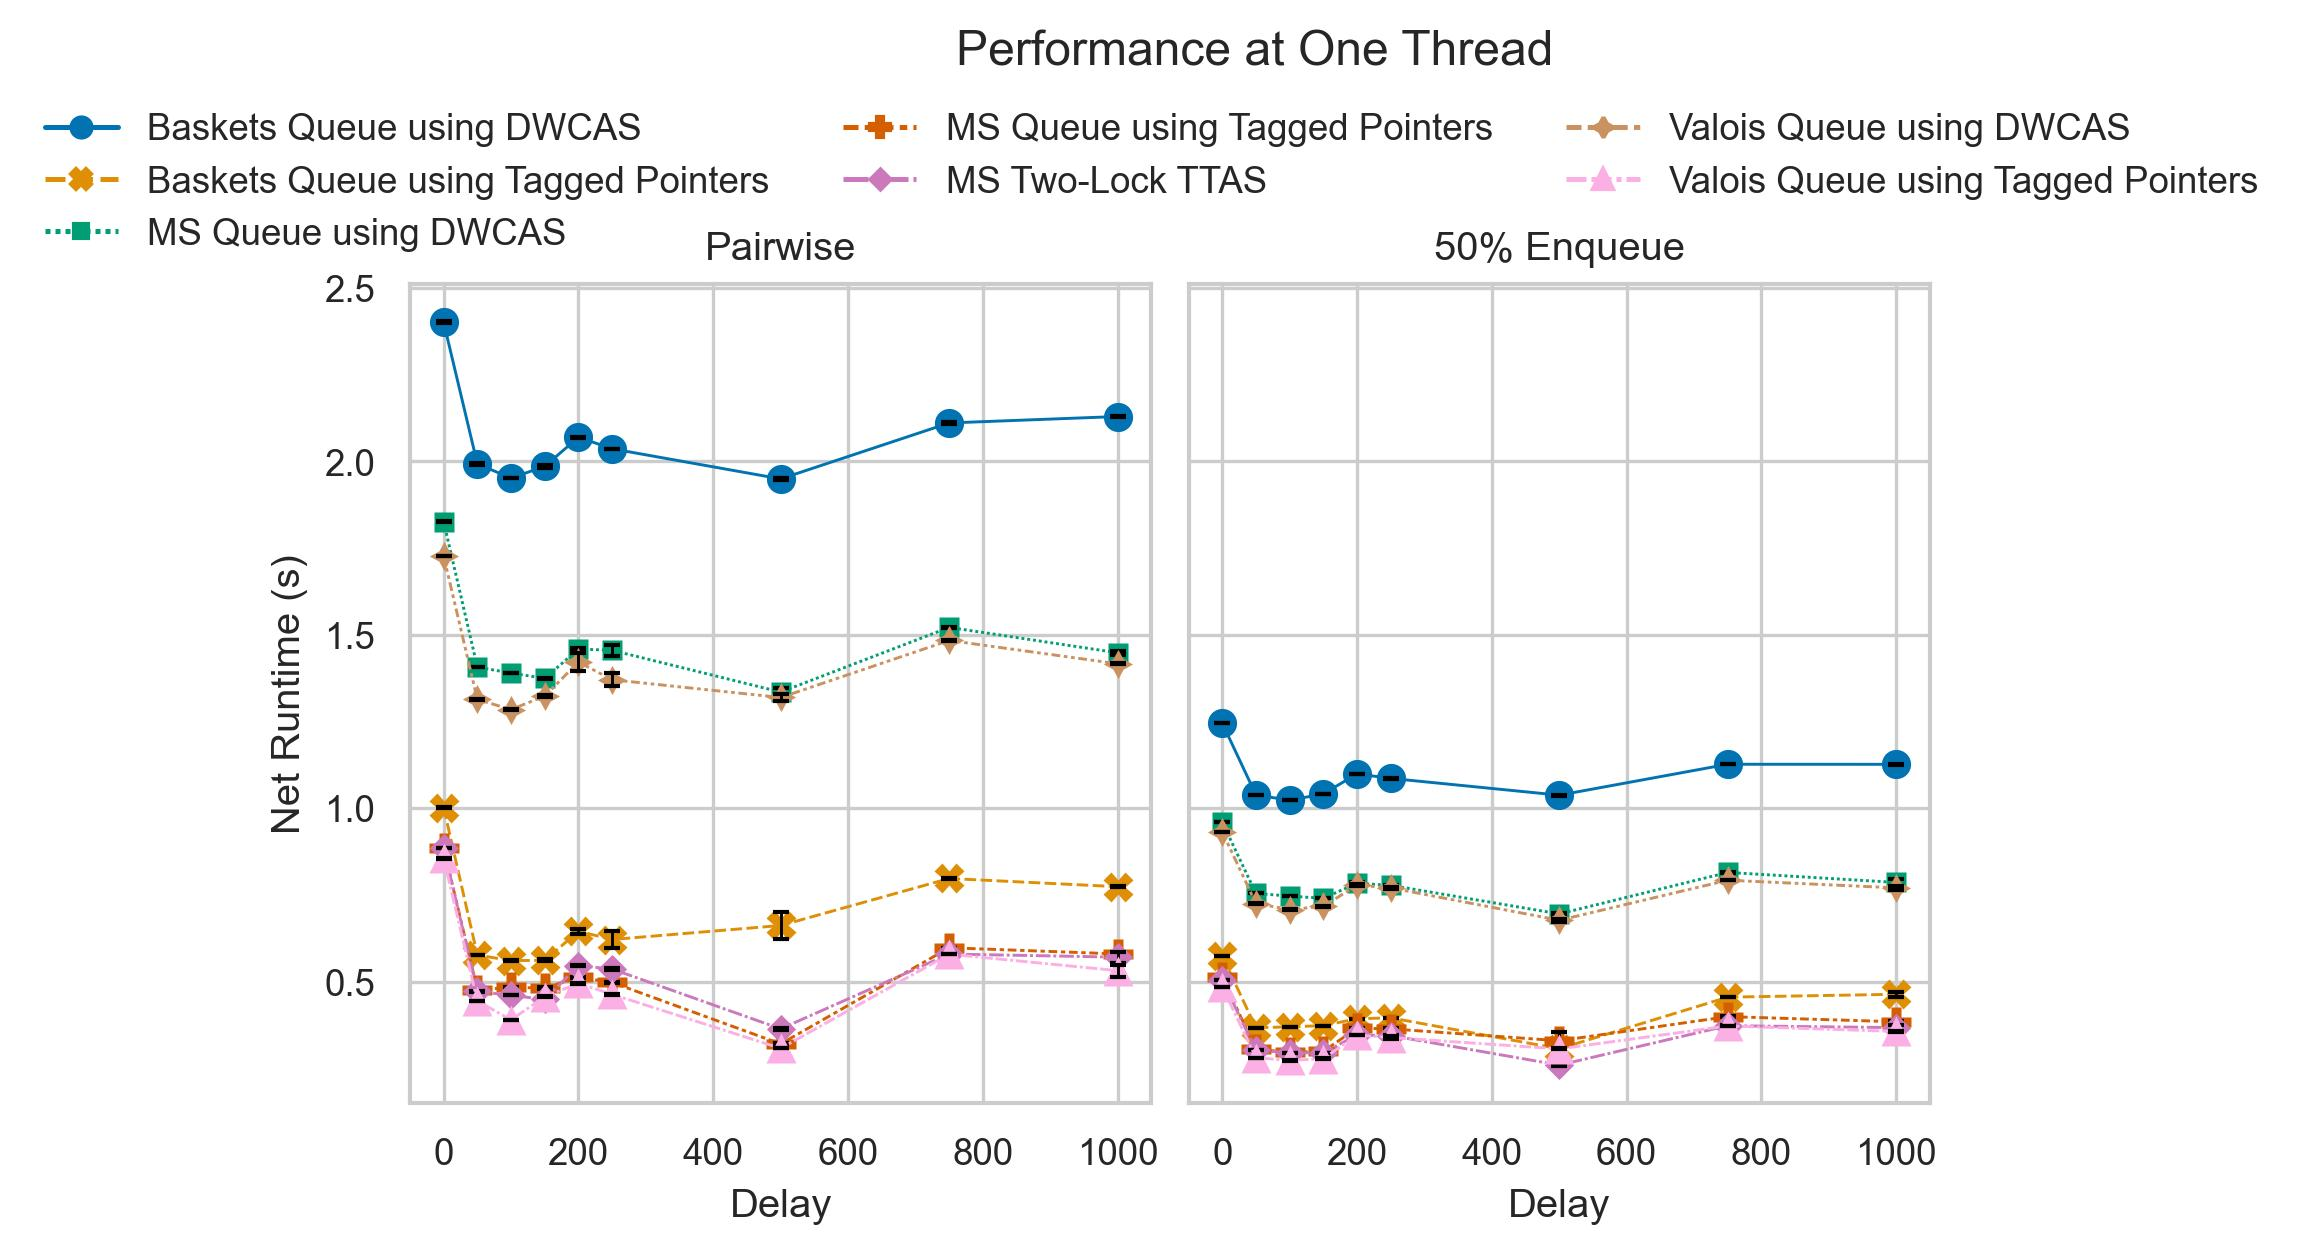
\includegraphics[width=1\textwidth]{plots/delay_thread_1.jpg}
    \caption{The pairwise and the 50\% benchmarks on the left and right respectively.}
    \label{fig:perf_1_thread}
\end{figure}

The sequential latency of a queue is determined by its algorithmic
complexity~\citep{valois1995datastructures}. Contention-reducing
mechanisms\textemdash such as thread helping\textemdash are not triggered under
single threaded workloads as they rely on failed CAS operations, adding
extra overhead through the computation of predicates.
Figure \ref{fig:perf_1_thread} shows the performance of each queue in a single
threaded workload. Under the \emph{pairwise benchmark}, the \emph{MS-Queue} and
the \emph{Baskets Queue} using tagged pointers are at most \textbf{3.168} and
\textbf{2.593} times faster than their DWCAS counterparts. 
The \emph{Baskets Queue} is consistently outperformed by the \emph{MS-Queue}
and the \emph{Two-Lock Queue} (respectively, at most \textbf{0.450} and
\textbf{0.516} times slower). Although the \emph{pairwise benchmark} does not
show which queue is consistently faster, the \emph{50\% enqueue benchmark}
shows that the \emph{Two-Lock Queue} consistently outperforms the
\emph{MS-Queue} (by at most \textbf{0.27} times).

\section{Workload under two threads}
Similar to \citep{michael1996simple,hoffman2007baskets,ladan2008optimistic},
under a workload of two threads, a significant degradation in performance can
be observed. \citeauthor{michael1996simple} notes that as each queue's head and
tail are shared across two processors, cache misses are more frequent. 
Figure \ref{fig:perf_deg_1_thread} shows that queues using tagged pointers tend
to experience higher contention, consequently leading to worse performance. 
In support of this claim, the \emph{Baskets Queue using Tagged Pointers} with
50 nanoseconds of delay was \textbf{2.435} times more likely to re-attempt an
enqueue\footnote{This metric was gathered by incrementing an integer (found in
thread local storage) every time it repeated anything past line \emph{E03} of
the Baskets Queue.} than its DWCAS counterpart.

\begin{figure}[!ht]
    \centering
    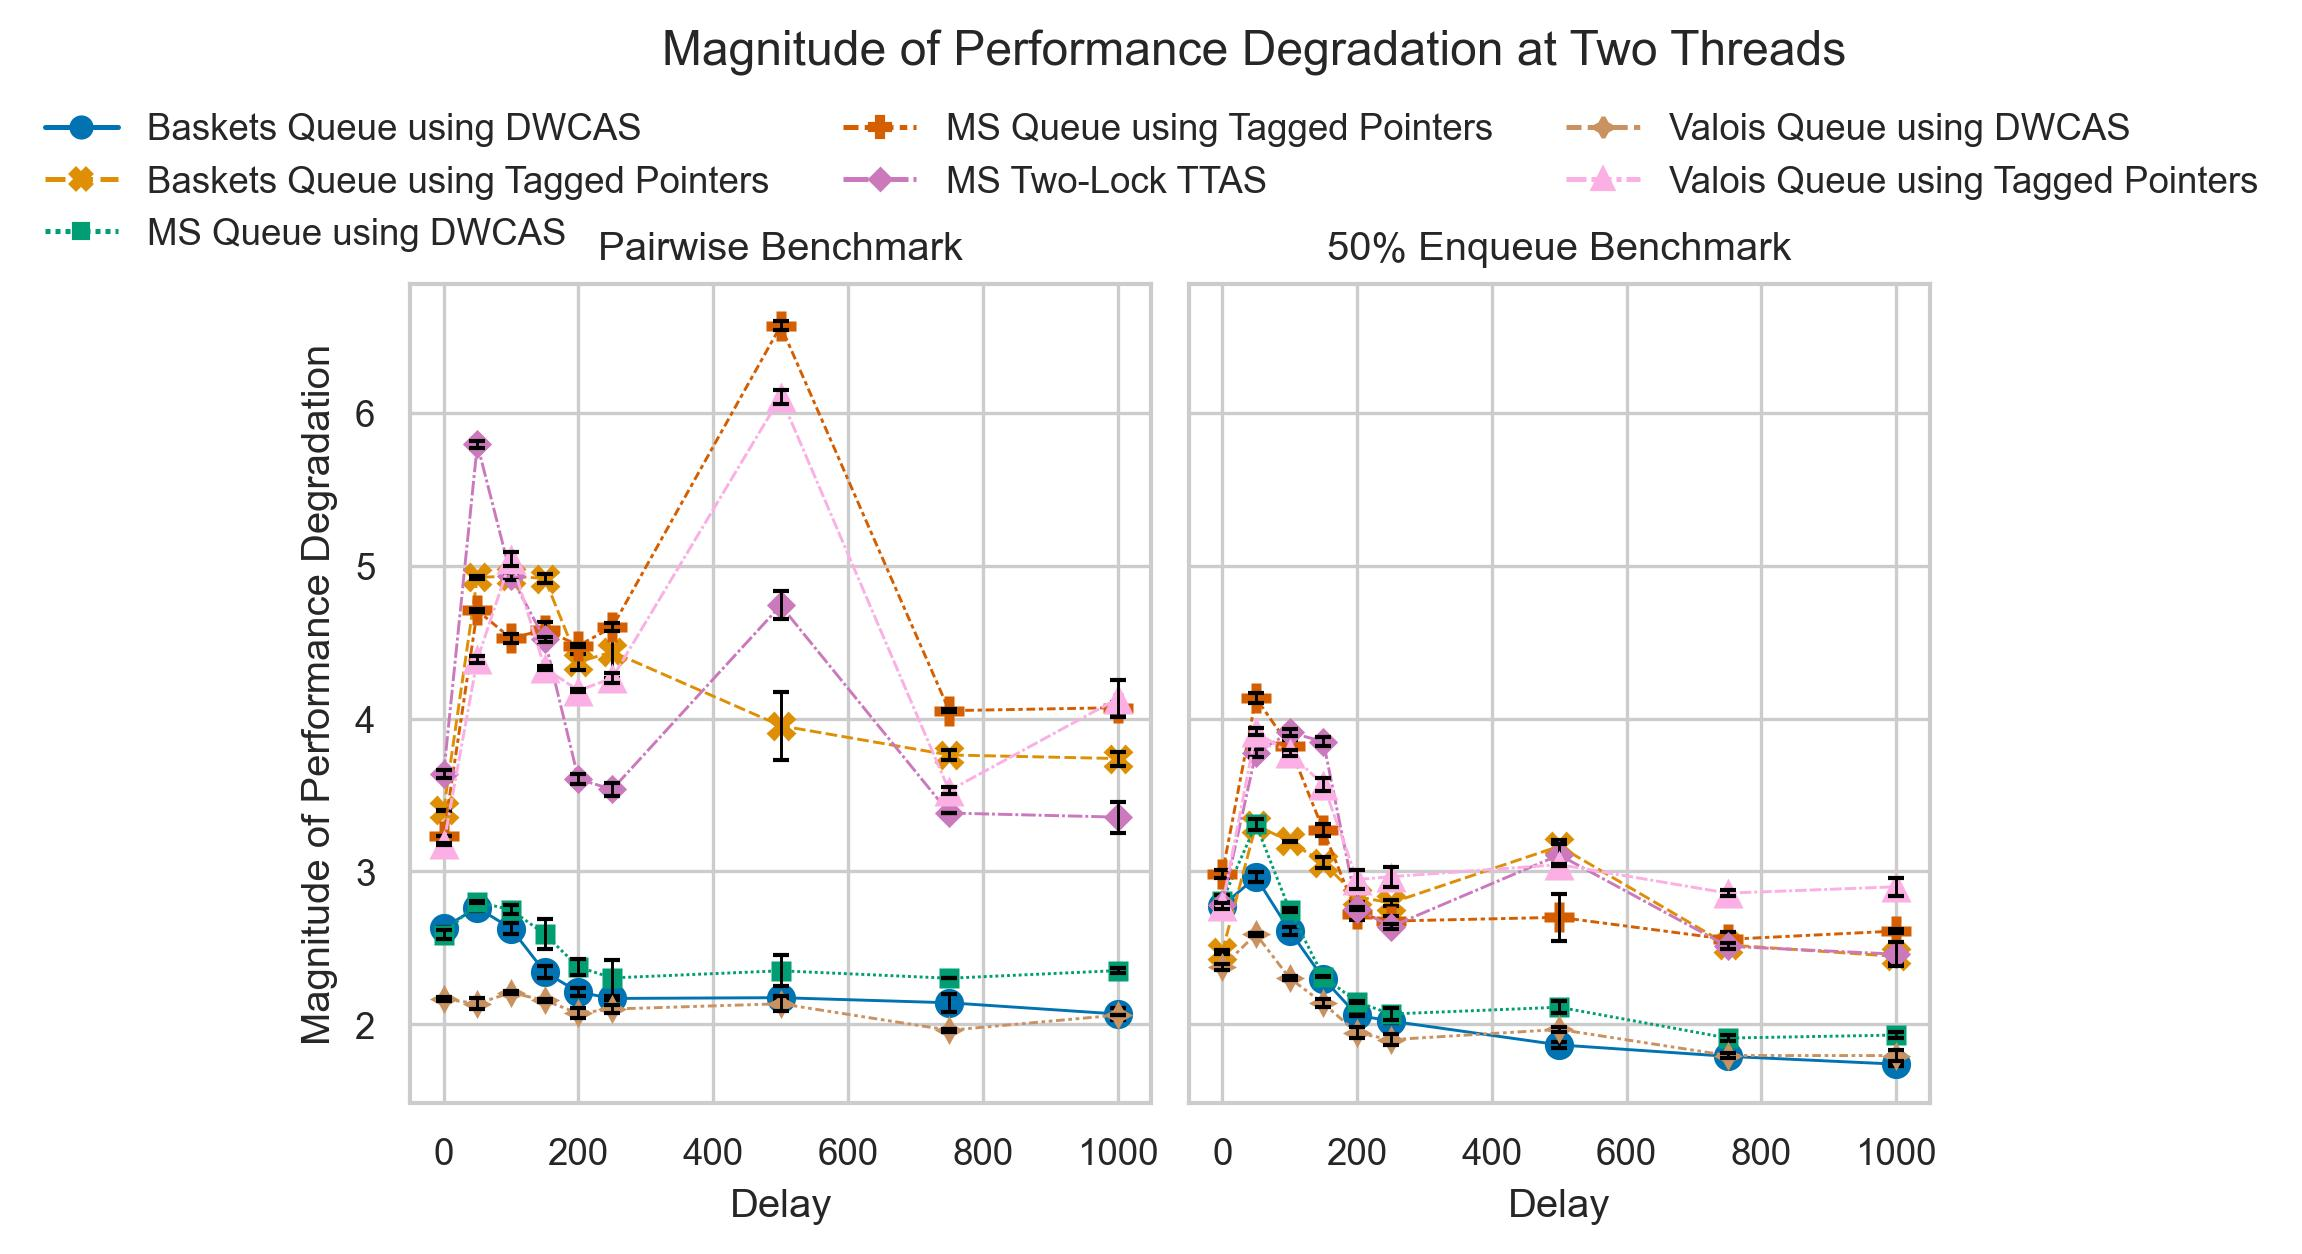
\includegraphics[width=1\textwidth]{plots/speedup_1.jpg}
    \caption{The magnitude of performance degradation between single and two-threaded workloads.}
    \label{fig:perf_deg_1_thread}
\end{figure}

\begin{figure}[!ht]
    \centering
    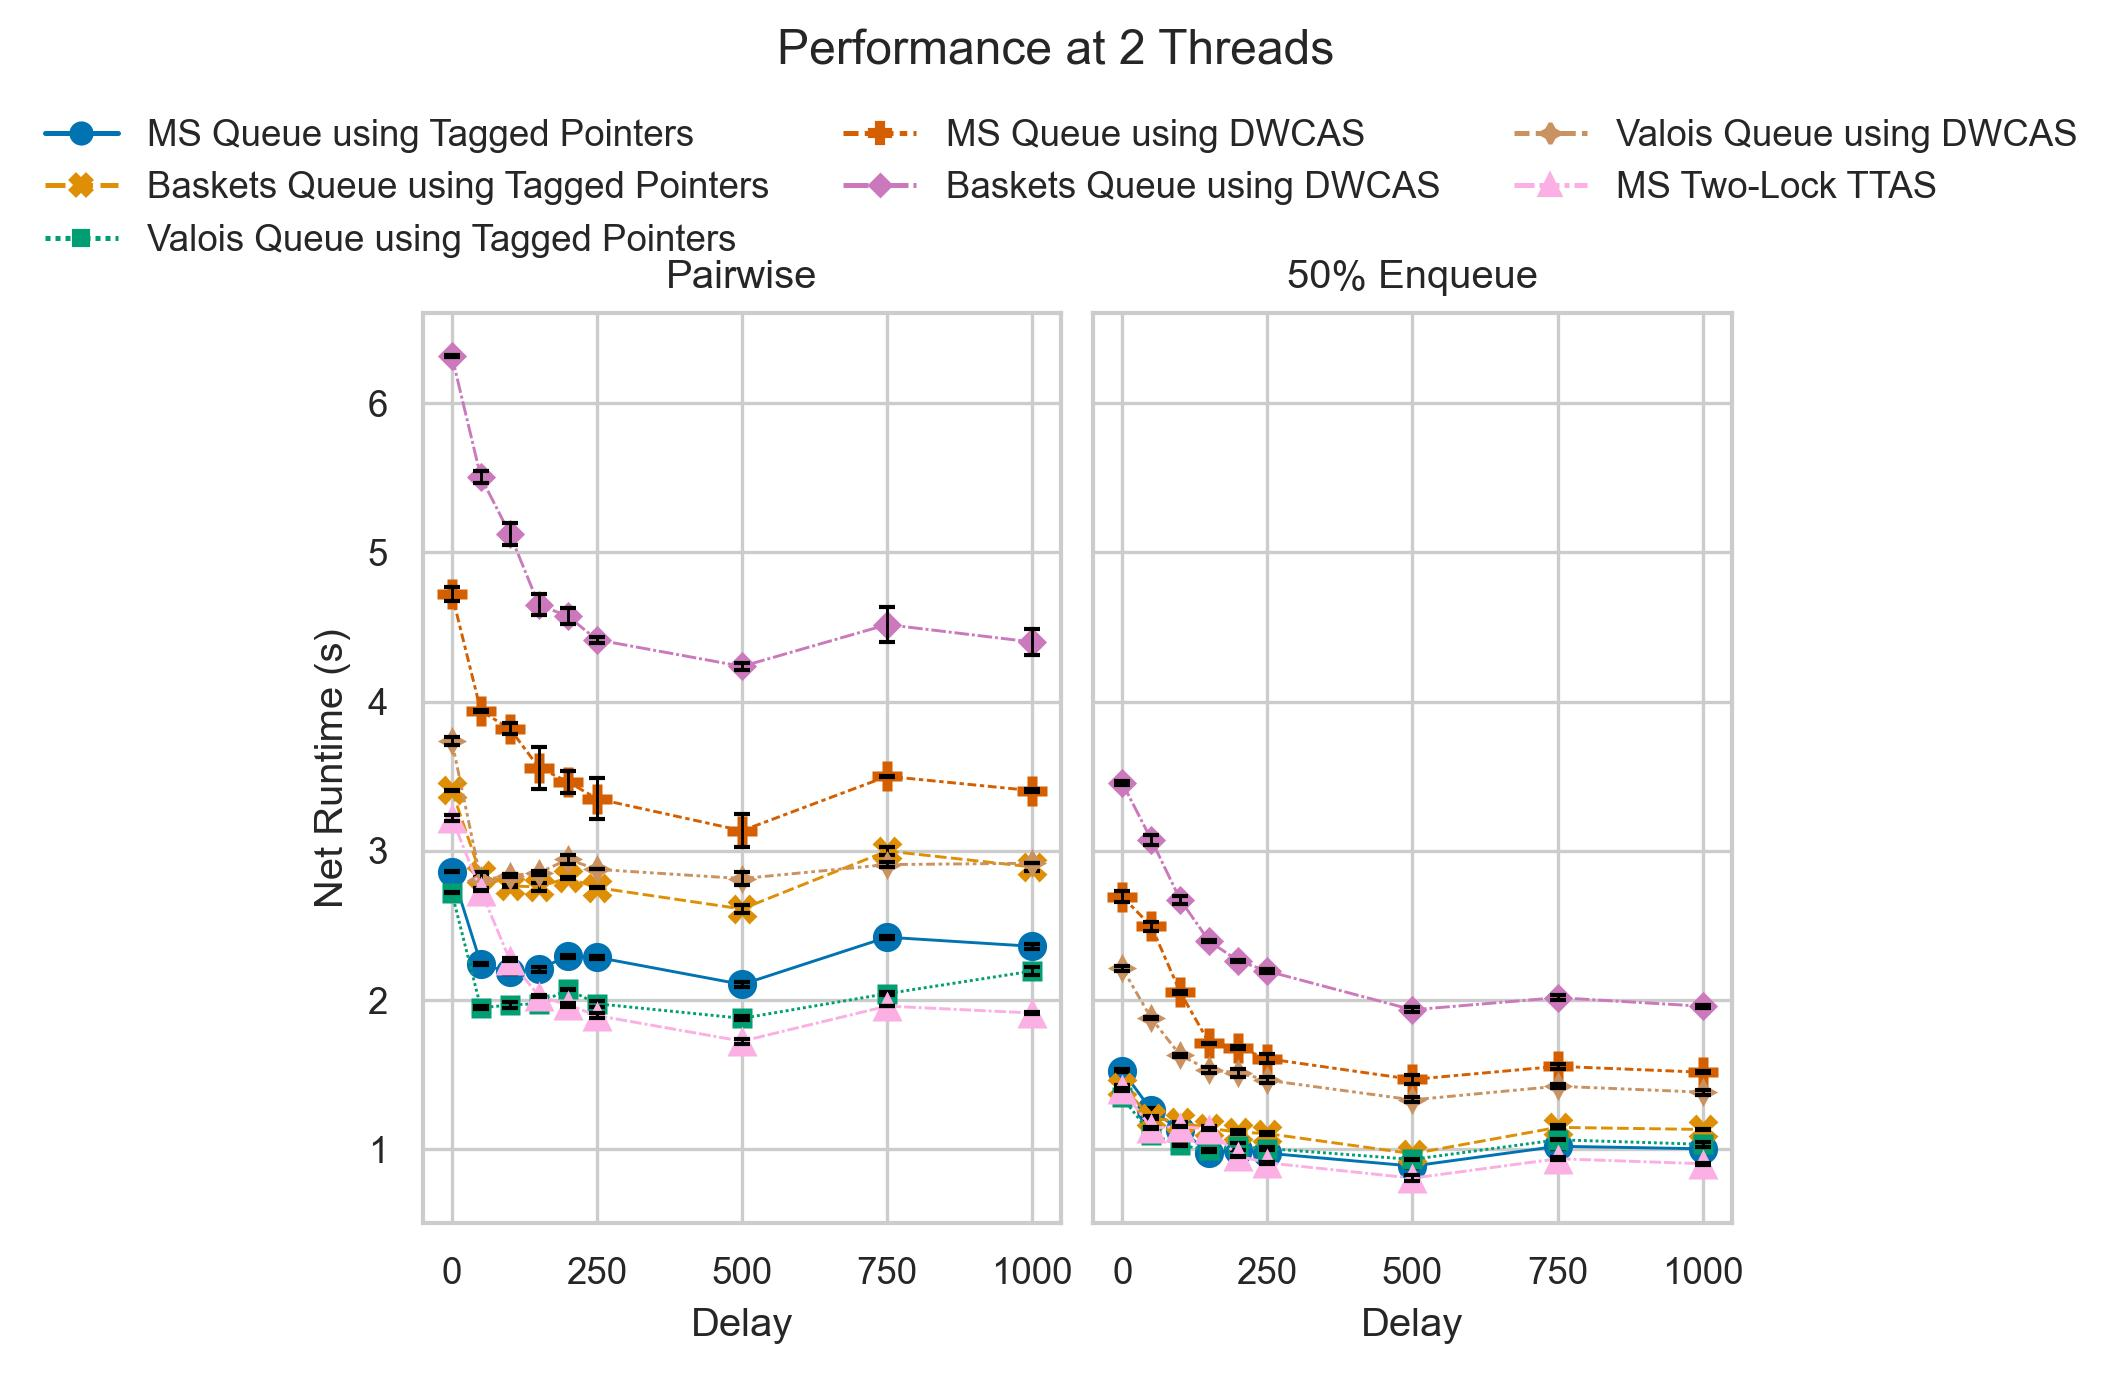
\includegraphics[width=1\textwidth]{plots/delay_thread_2.jpg}
    \caption{The pairwise and the 50\% benchmarks on the left and right respectively.}
    \label{fig:perf_2_thread}
\end{figure}

In the \emph{pairwise benchmark}, the \emph{Baskets Queue} is consistently
outperformed by the \emph{MS-Queue} and the \emph{Two-Lock Queue} by at most
\textbf{20.978\%} and \textbf{34.672\%}, with the \emph{Two-Lock Queue}
consistently outperforming the \emph{MS-Queue} by at most \textbf{11.100\%}.

At delays greater than 200 nanoseconds, the \emph{two-lock queue} exhibits the
best performance.
Although outperformed, non-blocking queues using tagged pointers remain
competitive under low-contention. 

The performance of \citeauthor{valois1994queues}' queue in this study highly
conflicts with that of \citep{michael1996simple}. Although a queue without a
memory reclamation scheme may share a common algorithm with one that has, it
does not imply that they are algorithmically equivalent, making their
performance unconnected; as this study does not include memory reclamation
schemes in its implementations, valid comparisons cannot be made with
~\citep{michael1996simple}'s results of \citeauthor{valois1994queues}' queue,
however, insights may still be inferred.
\citeauthor{michael1996simple} fail to disclose that their choice of
memory-reclamation schemes introduced a significant bias in favour of their
novel algorithms. 
This is only made clear when inspecting the study's published source
code~\citep{michael1996simple_sourcecode}, where \citeauthor{valois1994}' queue
makes use of the safe-read protocol, whilst the \emph{MS-Queue} only keeps
track of each threads' most recently recycled node non-atomically in thread
local storage.
% \citeauthor{michael1996simple} fail to disclose the memory
% reclamation scheme overheads used by each queue\textemdash which if discussed, would
% have made the fact that the \emph{MS-Queue} made use of a significantly simpler
% and less effective memory reclamation scheme than any other queue, leading to
% heavily biased comparisons in favour of the \emph{MS-Queue}.

One may hypothesize \citeauthor{valois1994queues}' queue fitted with the \emph{safe read}
protocol leads to a horribly inefficient algorithm, as each enqueueing thread
is required to traverse a number of nodes in the linked list, incurring a high
number of cache misses due to the reference counting system incurring
additional loads and stores on visiting and moving on from a node.

Figure~\ref{fig:perf_deg_2_thread} shows that at specific delays, speedups of
up to \textbf{6.591\%} can be obtained.
\citeauthor{michael1996simple} observe speedups of a factor less than
$\frac{1}{3}$~\citep{michael1996simple}, which is far more drastic than that
observed in \citep{ladan2008optimistic, hoffman2007baskets} and this study. The
50\% enqueue benchmark does not exhibit any speedups, further highlighting the
effects of a benchmark's artificiality on the validity of its results.

\section{Workload Under Three Threads}
A minor speedup under a workload of three threads is commonly
observed\citep{ladan2008optimistic,michael1996simple,hoffman2007baskets}.
\citeauthor{michael1996simple} link the boost in performance to fewer
iterations per thread, in combination with a cache miss rate similar to that
under two threads.

\begin{figure}[!ht]
    \centering
    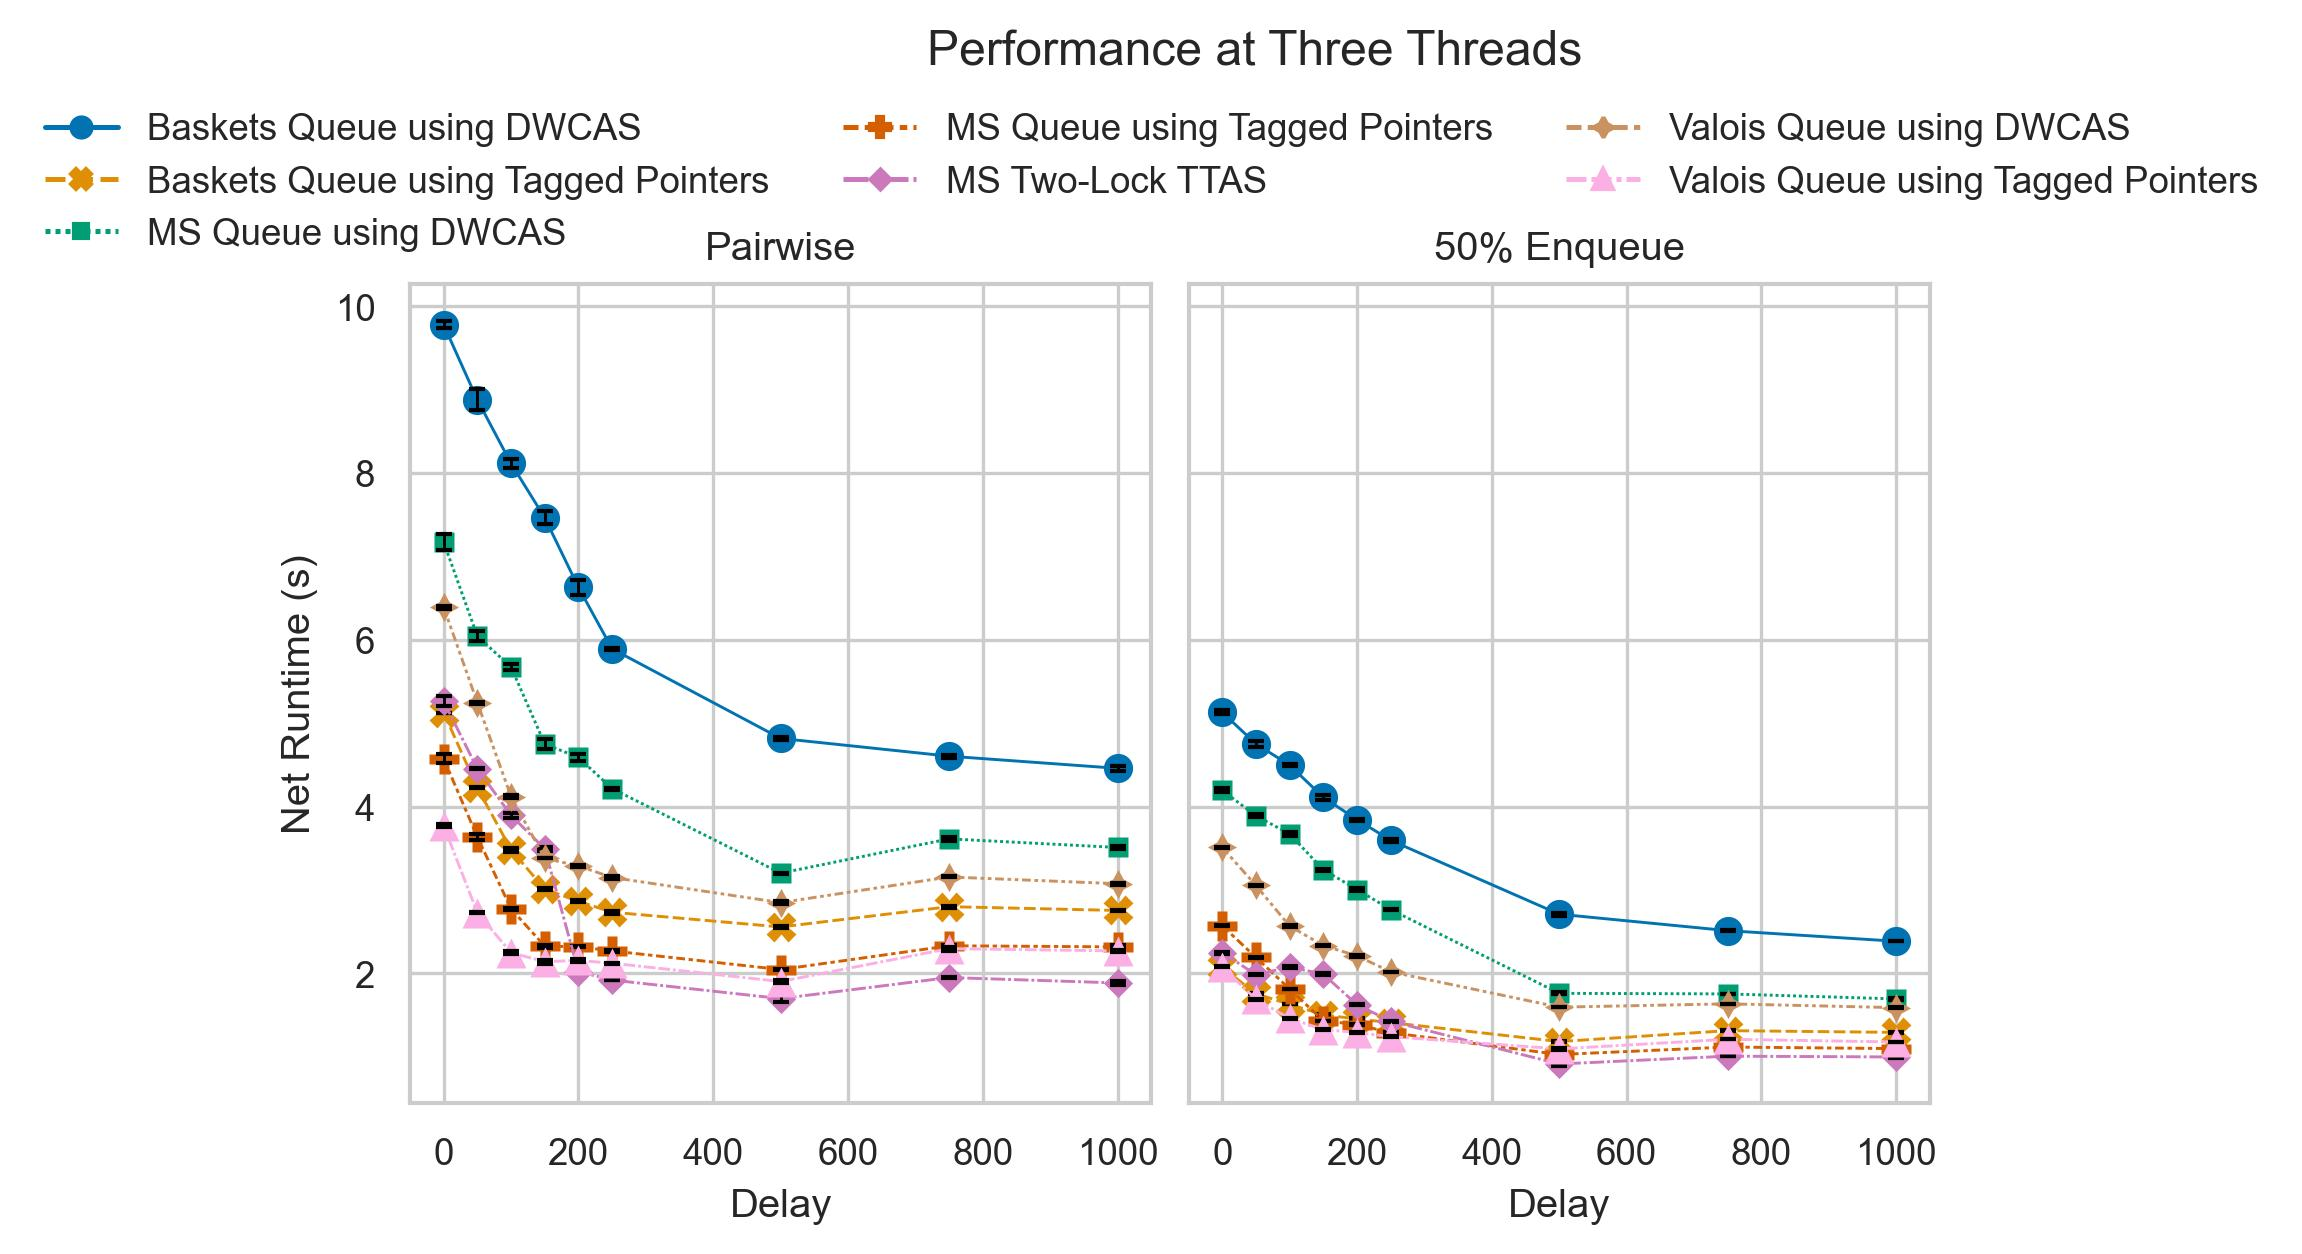
\includegraphics[width=1\textwidth]{images/plots/delay_thread_3.jpg}
    \caption{The pairwise and the 50\% benchmarks on the left and right respectively.}
    \label{fig:perf_3_thread}
\end{figure}


Up to delays of 150 nanoseconds, every non-blocking queue using tagged pointers
significantly outperforms the two-lock queue (\emph{MS-queue} is
\textbf{33.412\%} faster than the two-lock queue at 150 nanoseconds of delay),
however, as contention drops, the two-lock queue tends to become favourable. 
The \emph{MS-queue} consistently outperforms the \emph{Baskets Queue} by at least
\textbf{10.778\%}.
As the degree of contention under three threads is higher than that at two
threads, the performance penalty in using higher delays is reduced.

\begin{figure}[!ht]
    \centering
    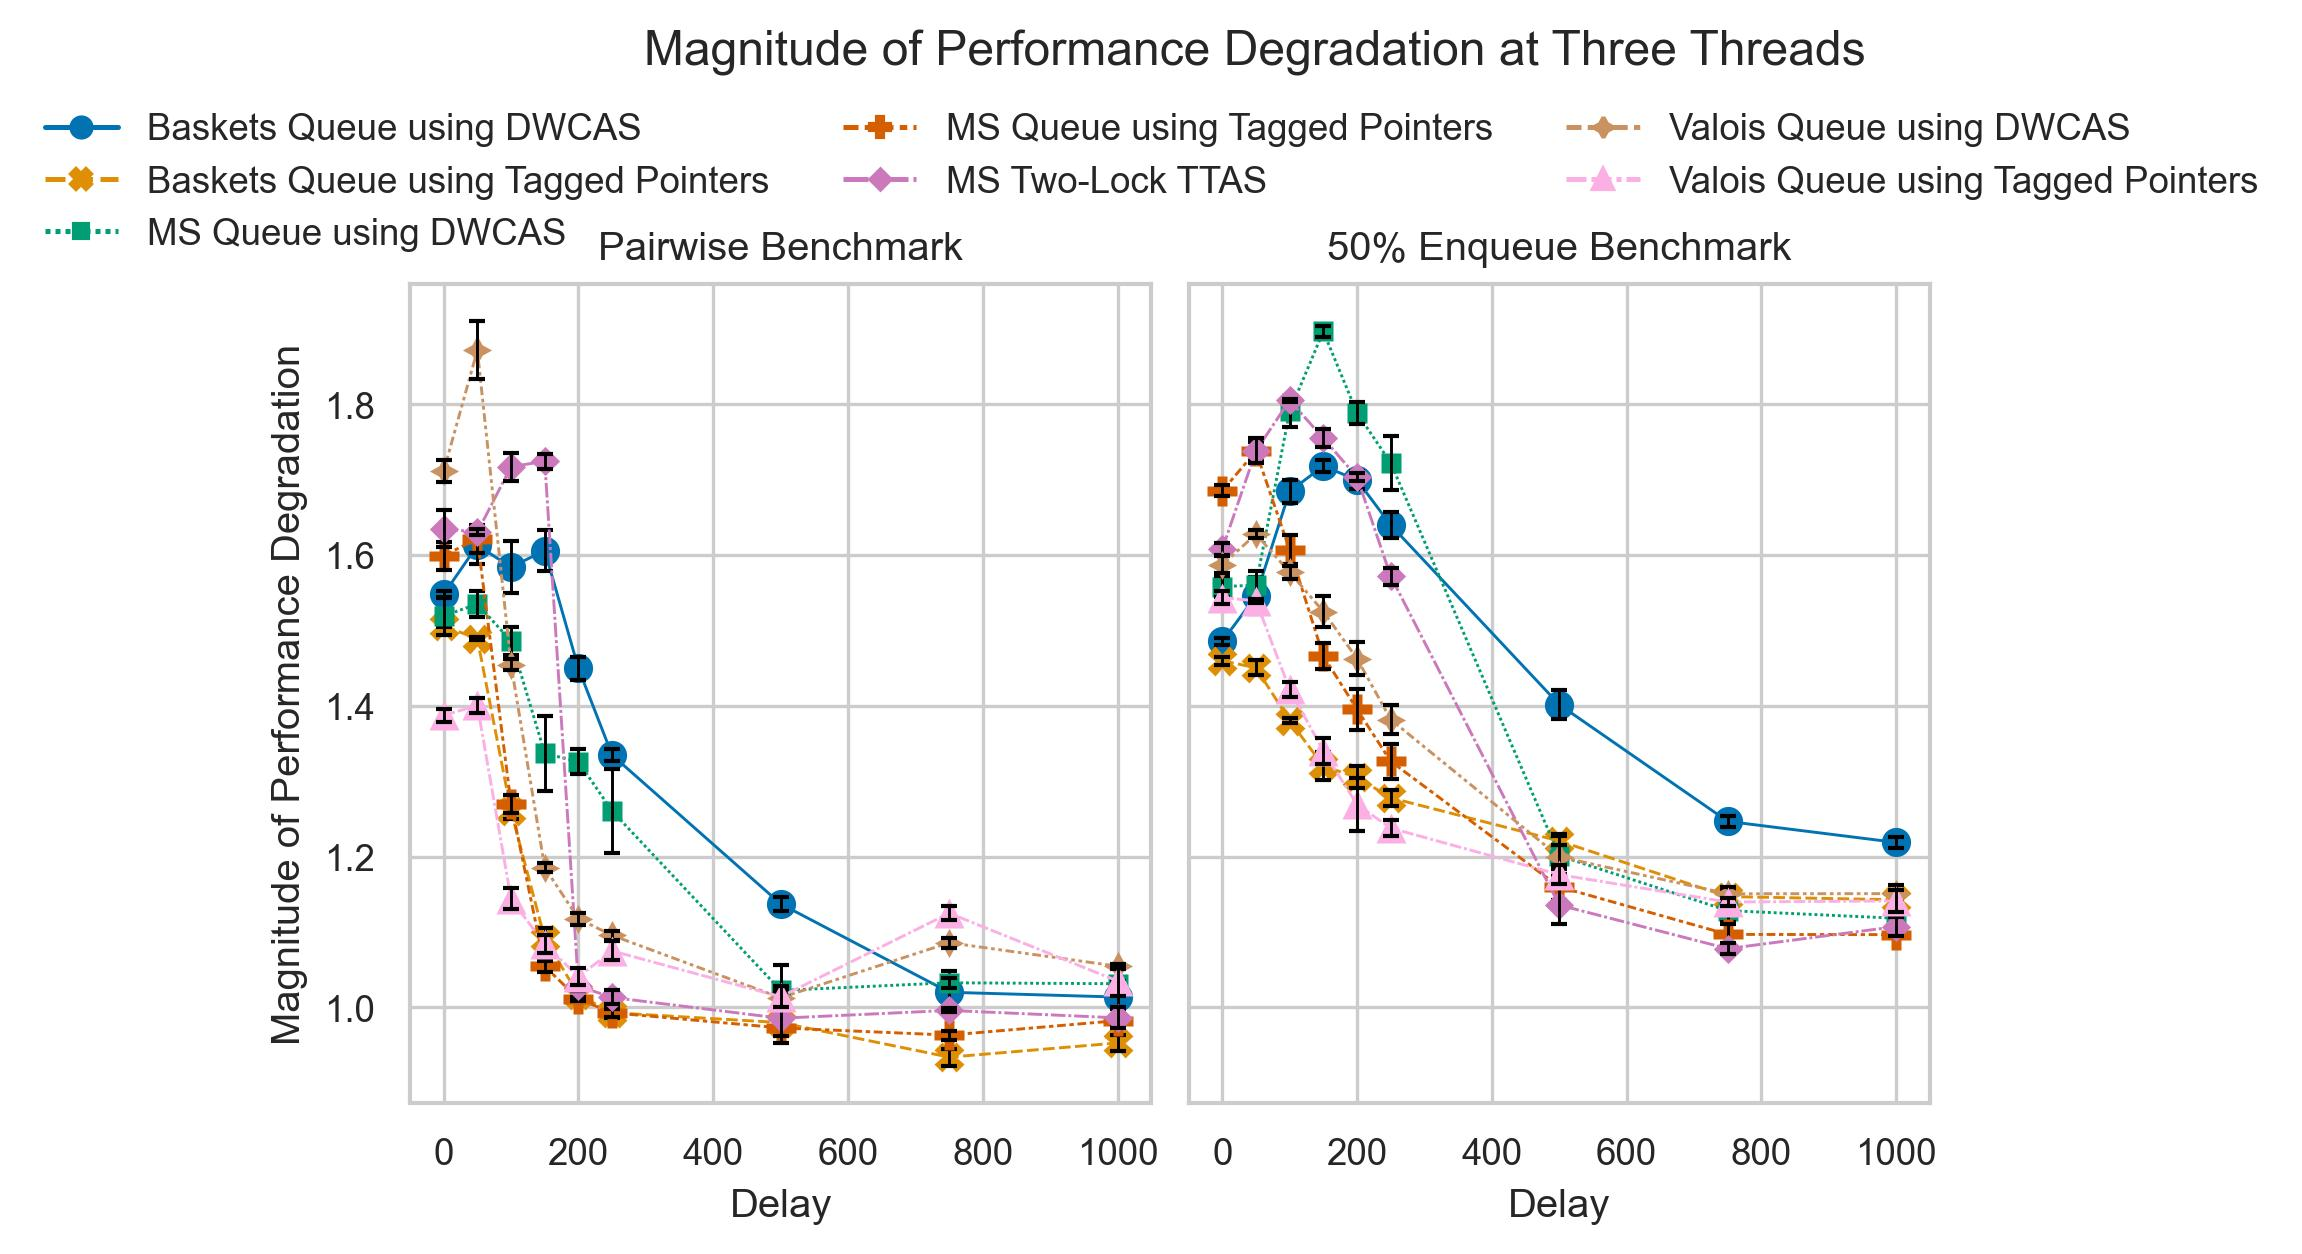
\includegraphics[width=1\textwidth]{images/plots/speedup_2.jpg}
    \caption{The pairwise and the 50\% benchmarks on the left and right respectively.}
    \label{fig:perf_deg_2_thread}
\end{figure}

\section{Workload Under Four Threads\label{sec:workload_four_threads}}

At four threads,
\citep{michael1996simple,hoffman2007baskets,ladan2008optimistic} observe a
slight dip in performance for both the \emph{MS-queue} and the \emph{Two-Lock
Queue}.
\citeauthor{hoffman2007baskets} notes an increase in performance for the
\emph{Baskets Queue}. As each queue at every delay exhibits a magnitude greater
than one, it can be concluded that performance has worsened.

Figure \ref{fig:perf_4_thread} shows that under the pairwise benchmark and no
delay, the \emph{Baskets Queue} is \textbf{0.259\%} slower than the \emph{MS-Queue};
At delays of 50 and 100 nanoseconds, the \emph{Baskets Queue} is
respectively \textbf{0.765\%} and \textbf{3.668\%} faster than the
\emph{MS-Queue}; Above delays of 100 nanoseconds, the \emph{Baskets Queue} is
up to \textbf{26.074\%} slower than the \emph{MS Queue}. 
On the other hand, the \emph{50\% Enqueue Benchmark} shows that the
\emph{Baskets Queue} is up to \textbf{42.047\%} faster than the
\emph{MS-Queue}. The distinct characteristics of the \emph{50\% Enqueue
Benchmark} allowed for the \emph{Baskets Queue} to make use of the baskets
thread-helping mechanism up to \textbf{110.964} times more than in the
\emph{Pairwise Benchmark}.
\citeauthor{hoffman2007baskets} use a variation of
\citeauthor{michael1996simple}'s \emph{pairwise benchmark}, where each thread
alternates between enqueues and dequeues. It is possible that this variation
was purposely chosen, as the alternation of operations creates an environment
where the \emph{`baskets'} mechanism is used more frequently.

% \citeauthor{hoffman2007baskets} use a variation of
% \citeauthor{michael1996simple}'s \emph{pairwise benchmark} where each thread
% alternates between executing an enqueue or a dequeue. It is possible this
% variation was purposely adopted, as the alternating execution of operations
% creates an environment where the \emph{baskets mechanism} is used more
% frequently.

\begin{figure}[!ht]
    \centering
    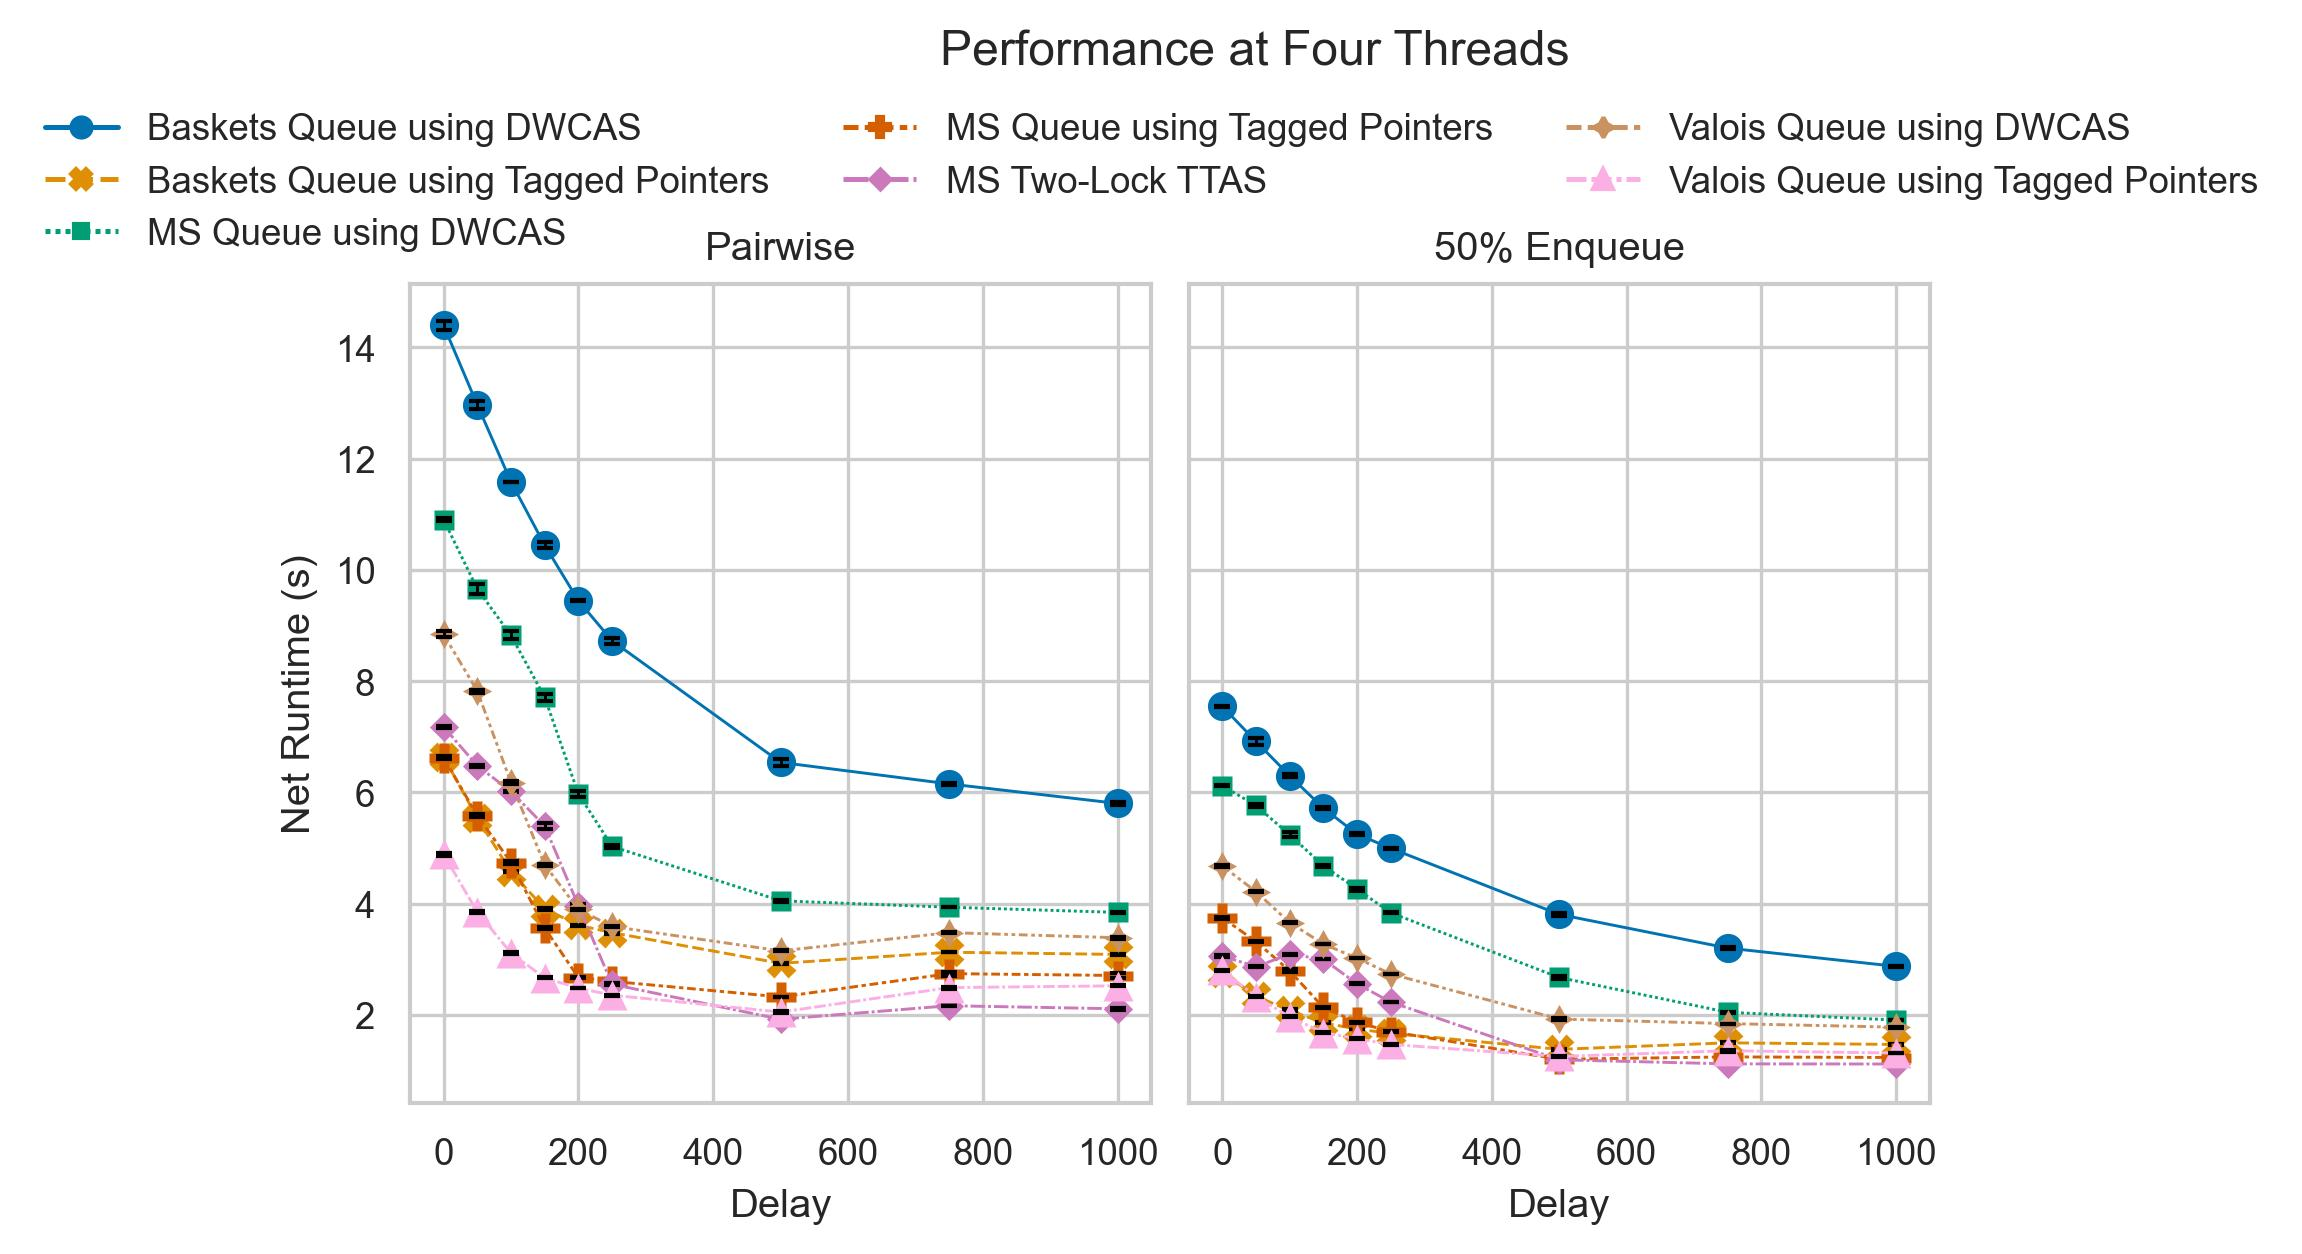
\includegraphics[width=1\textwidth]{images/plots/delay_thread_4.jpg}
    \caption{Pairwise and 50\% Enqueue Benchmarks at four threads.}
    \label{fig:perf_4_thread}
\end{figure}

\begin{figure}[!ht]
    \centering
    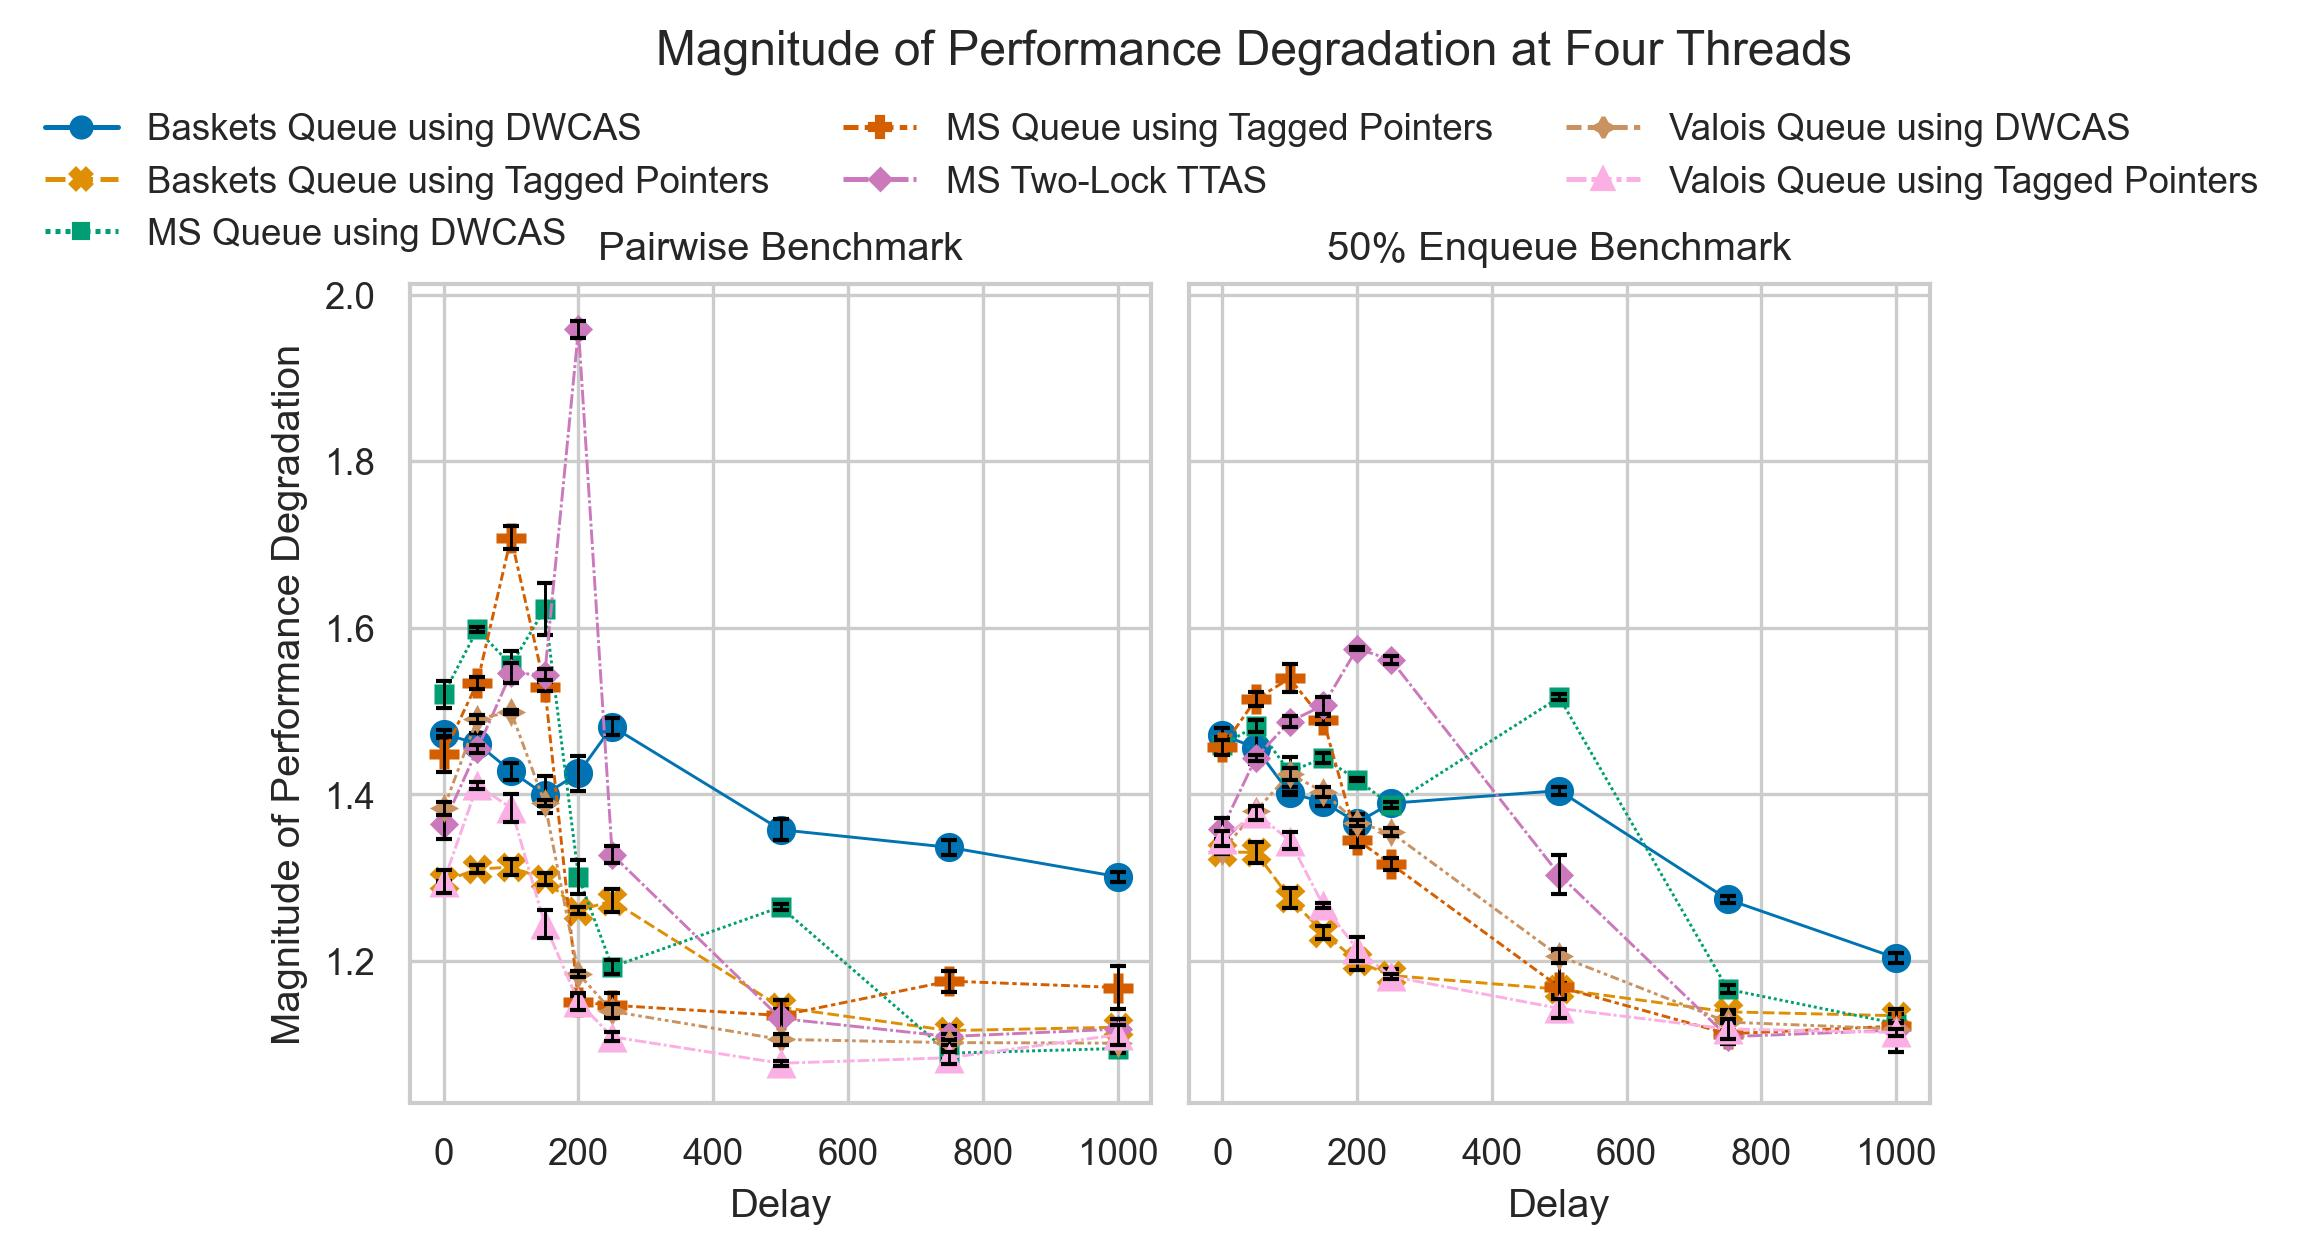
\includegraphics[width=1\textwidth]{images/plots/speedup_3.jpg}
    \caption{Degree of performance degradation at four threads.}
    \label{fig:perf_deg_4_thread}
\end{figure}

\pagebreak

\section{Performance Under Oversubscription}
\subsection{Workload Under Five Threads}
In this study, processors are oversubscribed by pinning more than one process
to each processor, forcing the thread scheduler to increase the frequency of
context-switches.

Figure \ref{fig:perf_deg_5_thread} shows that between 0 and 150 nanoseconds of delay, the
magnitude of performance degradation is a linear function of delay; As delays
greater than 150 nanoseconds are used, performance degradation explodes.
One may hypothesize that the sudden explosion in performance degradation is a result of
the significantly decreased time between context switches; as delay increases, 
the total CPU time available is further reduced.

In the pairwise benchmark, between 0 and 250 nanoseconds of delay, the \emph{Baskets
Queue} and the \emph{MS-Queue} are at most
\textbf{47.045\%} and \textbf{60.604\%} faster than the \emph{two-lock queue};
Between 500 and 1000 nanoseconds, the \emph{two-lock queue} is at most \textbf{3.351\%}
faster than the baskets queue.

Similar to the trends observed in section \ref{sec:workload_four_threads}, the \emph{Baskets
Queue} significantly outperforms the \emph{MS-Queue} (by at most \textbf{53.645\%}) only
in the \emph{50\% Enqueue Benchmark}. This repeating pattern shows that the performance of the
\emph{Baskets Queue} is heavily dependent on the utilization of the baskets mechanism.

\begin{figure}[!ht]
    \centering
    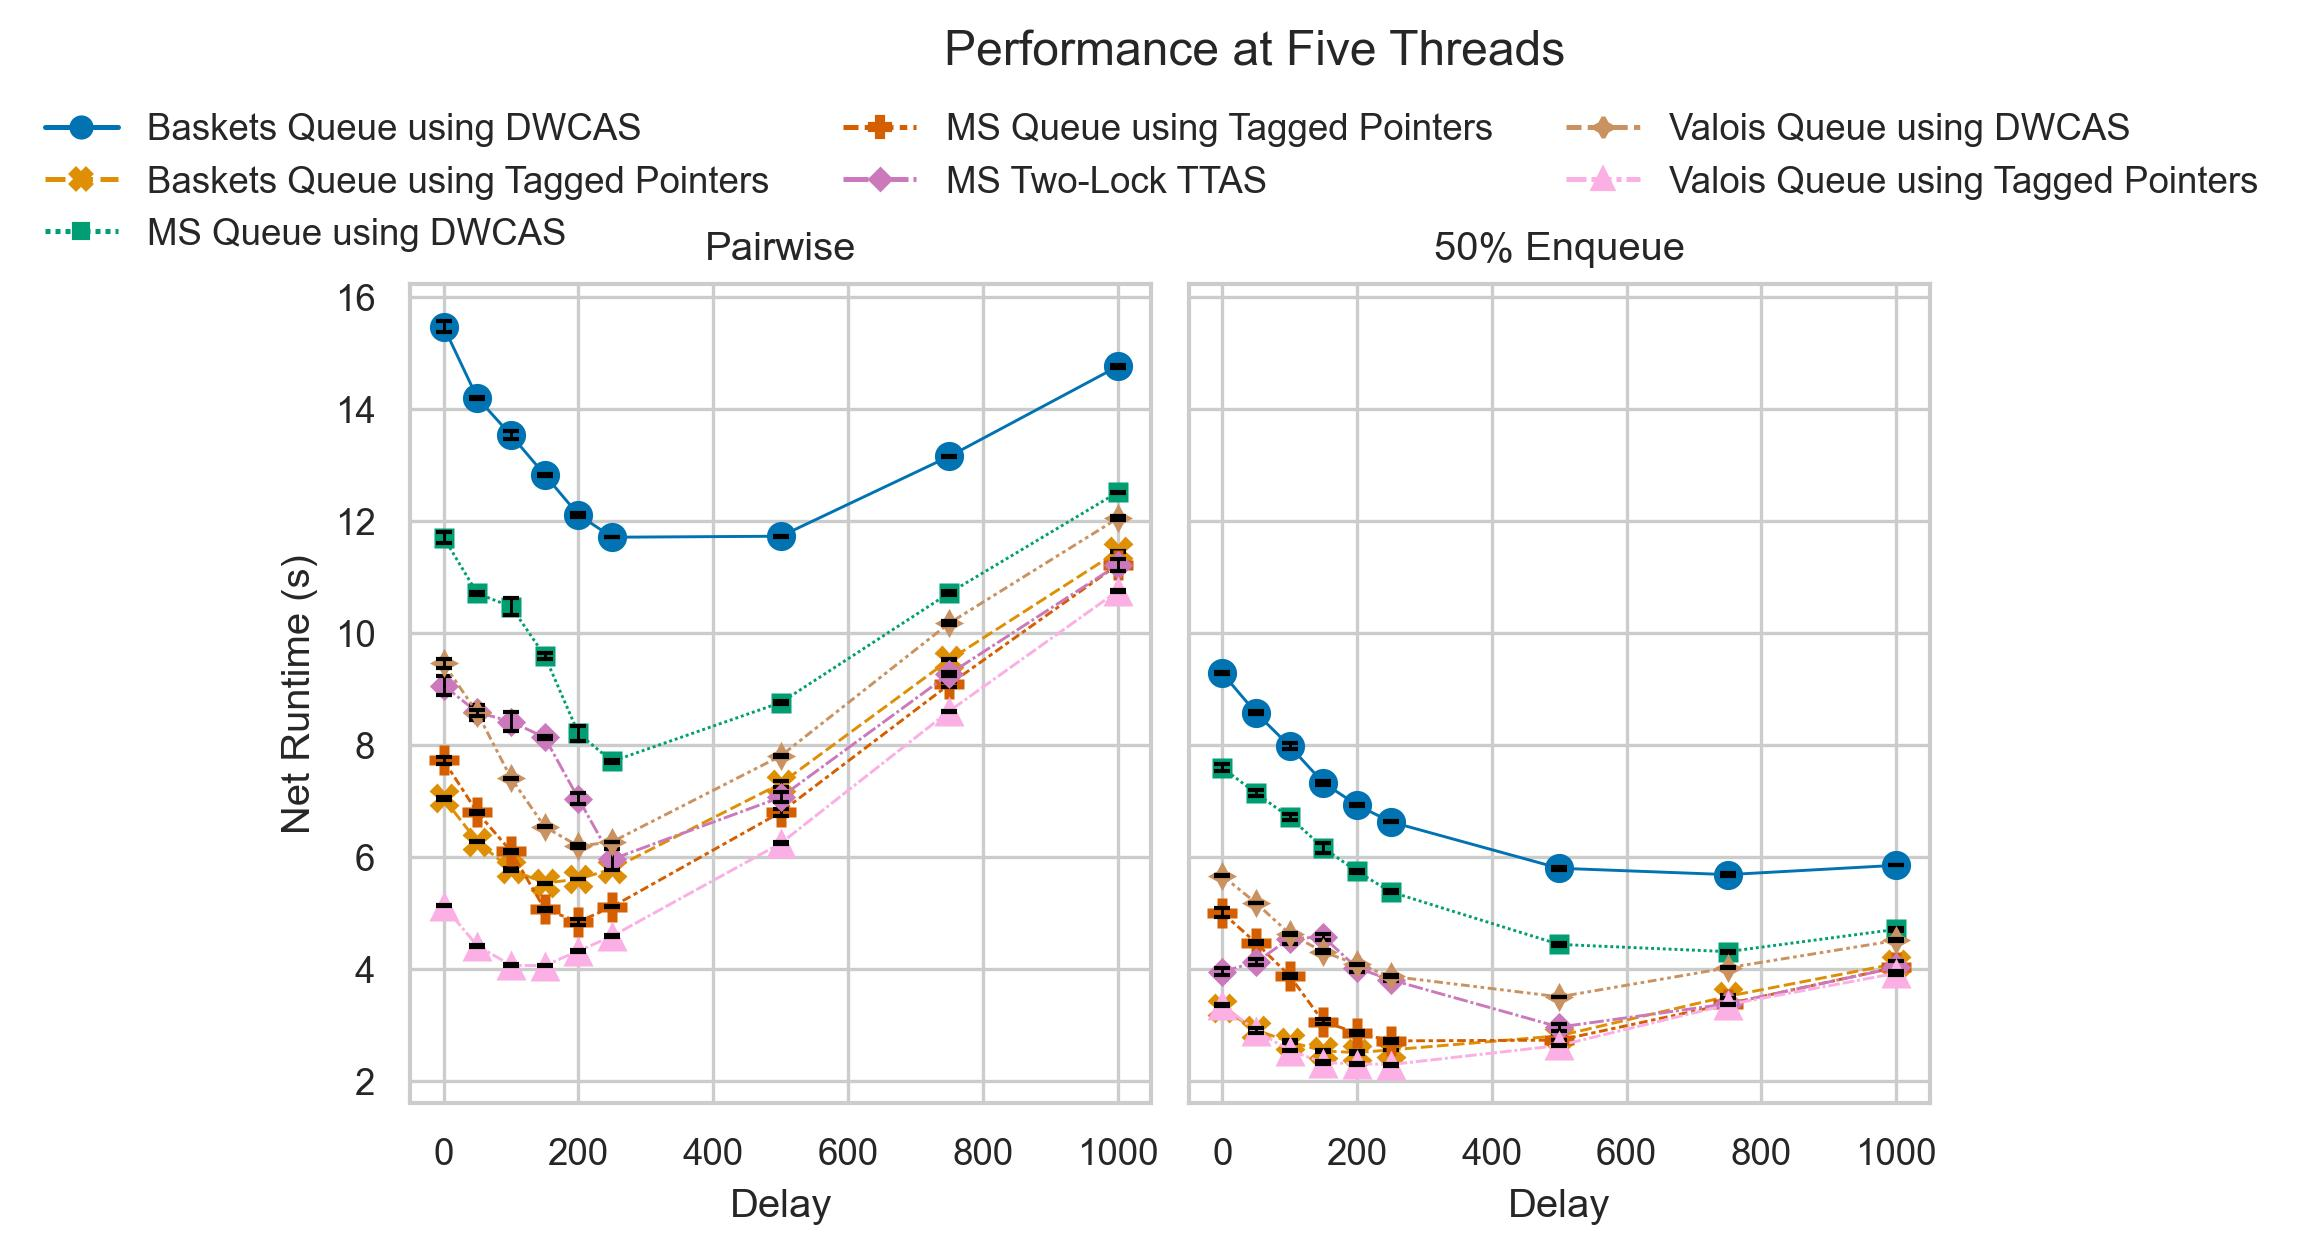
\includegraphics[width=1\textwidth]{images/plots/delay_thread_5.jpg}
    \caption{Pairwise and 50\% Enqueue Benchmarks at five threads.}
    \label{fig:perf_5_thread}
\end{figure}

\begin{figure}[!ht]
    \centering
    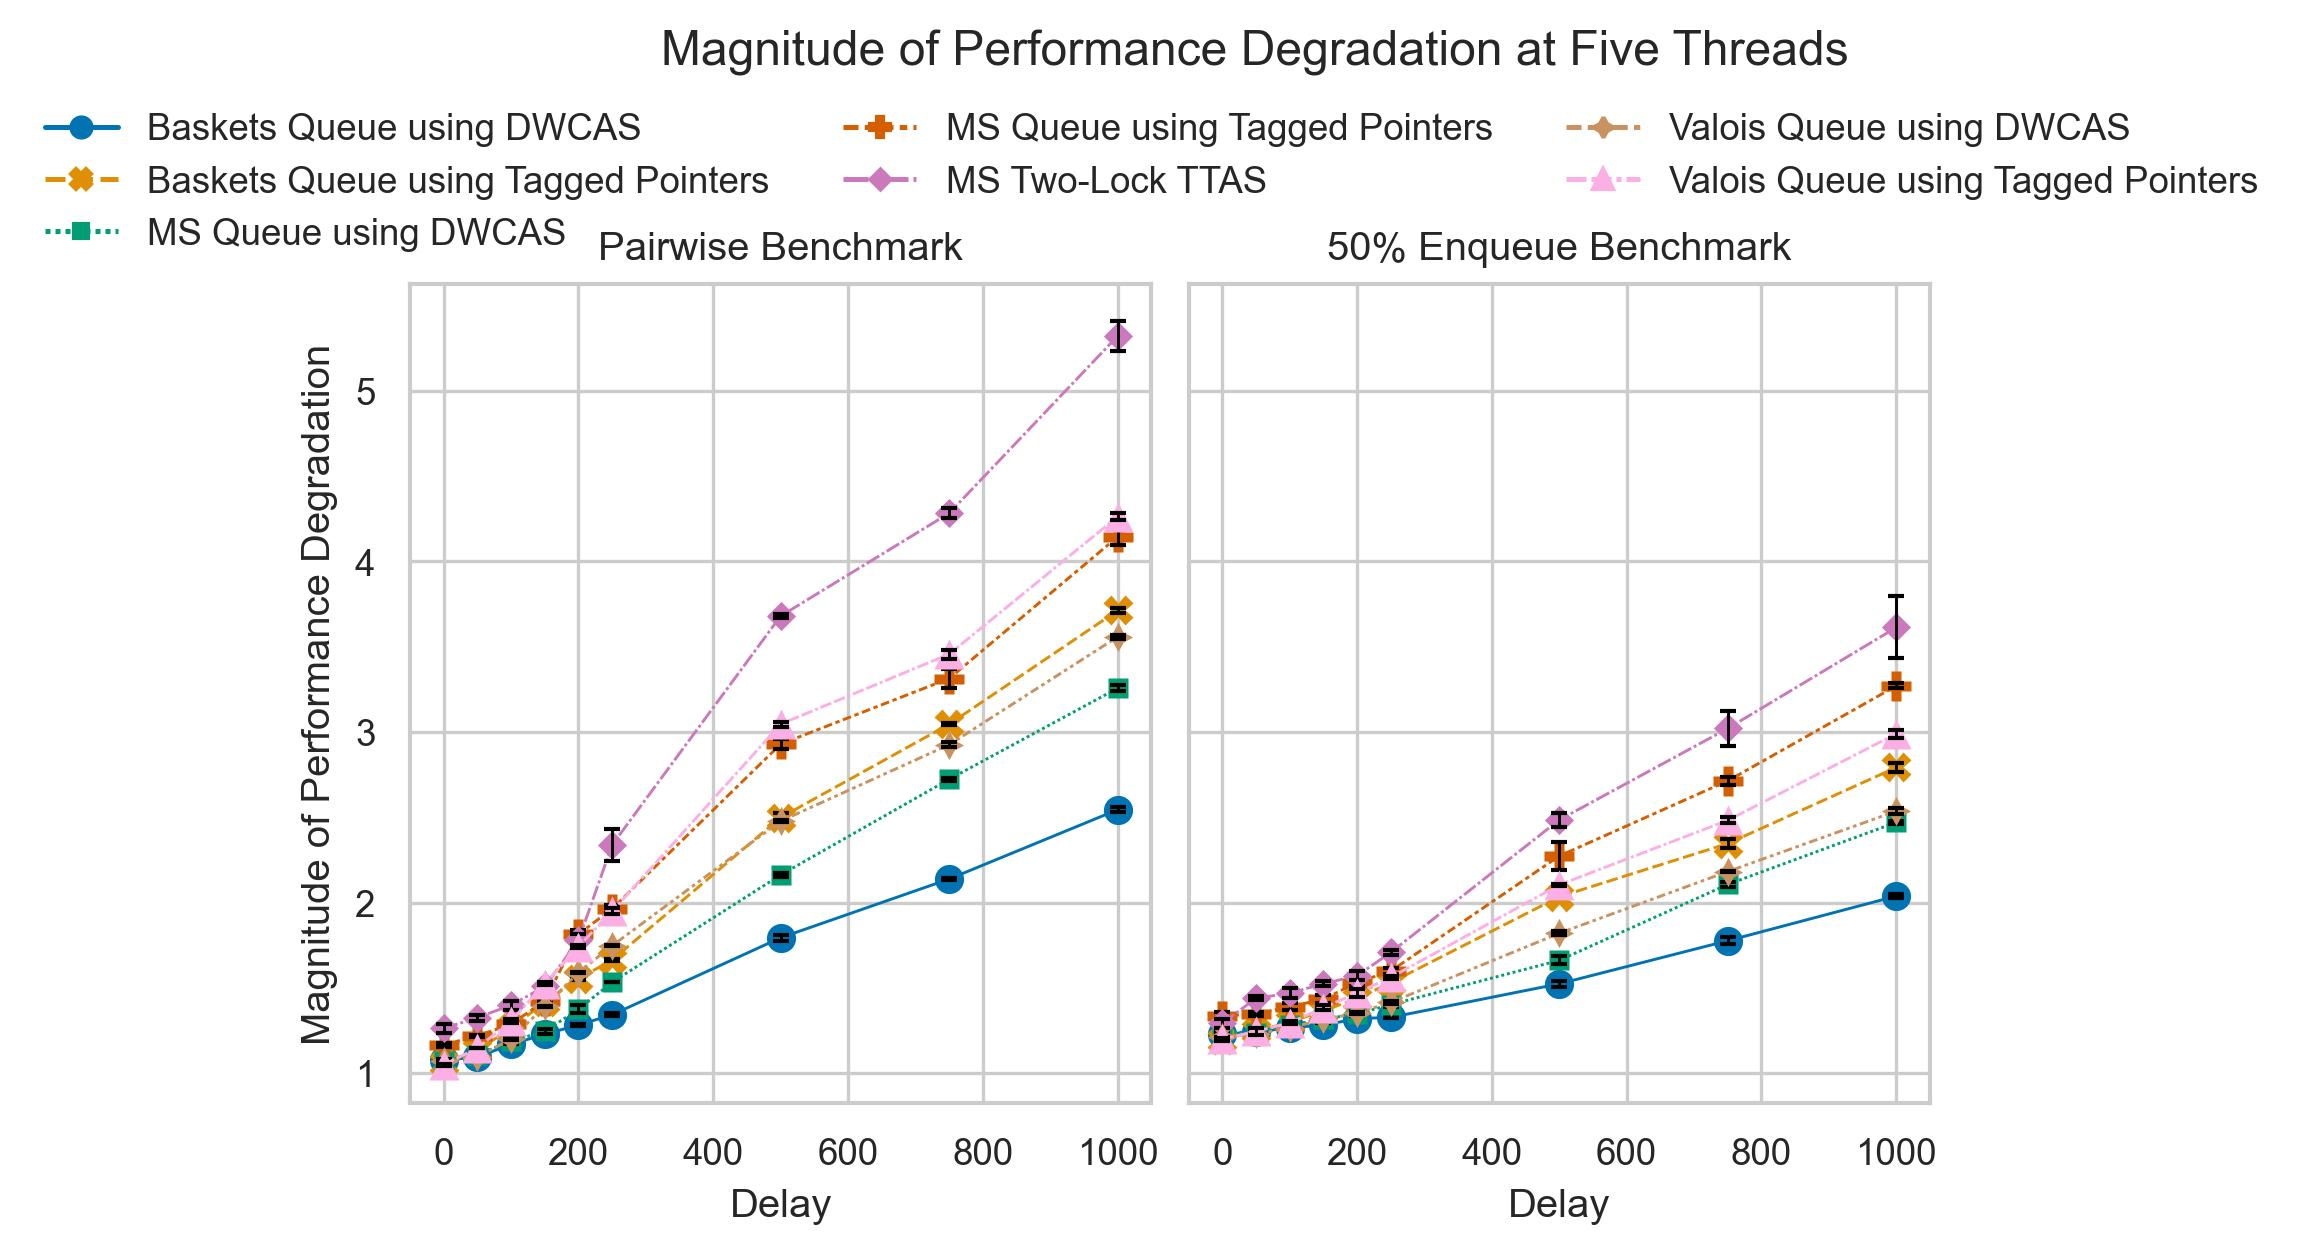
\includegraphics[width=1\textwidth]{images/plots/speedup_4.jpg}
    \caption{Degree of performance degradation at five threads.}
    \label{fig:perf_deg_5_thread}
\end{figure}

\subsection{Six Threads and Above}
At six threads, the non-blocking queues significantly outperform the \emph{two-lock}
queue at every delay. This trend repeats itself up to 12 threads, with the
degree at which the non-blocking queues outperform the \emph{two-lock queue}
increasing at every thread; the degree at which the \emph{baskets queue} outperforms
the \emph{MS-Queue} also grows with every thread.

\section{Effects of Delay on Performance}
\citeauthor{valois1995datastructures} and \citeauthor{hoffman2007baskets}
\citep{valois1995datastructures,hoffman2007baskets} note that backoff
algorithms are required to improve the efficiency of concurrent algorithms.
More often than not, a queue's optimal delay tends to be similar in consecutive
threads, with the pattern changing once over-subscription is present. Between
one and four threads, \textbf{$91.667\%$} (under the \emph{pairwise benchmark})
and \textbf{$83.333\%$} (under the \emph{50\% enqueue benchmark}) of all optimal net
runtimes have a delay of \textbf{500 nanoseconds}. Between five and twelve threads,
each queue's optimal delay slightly varies between zero and 250 nanoseconds. 

% \section{Effects of DWCAS on Concurrent Queues}
% From the data presented, one may note that employing the DWCAS instruction
% comes at a significant cost in performance. The performance penalty can be attributed to the
% latency of the DWCAS operation, leading to a lower number of operations being
% executed per second. It is possible that 

\section{Biases and Threats to Validity}
\paragraph{Artificiality of Workloads}
In \citep{gregg2014systems}, \citeauthor{gregg2014systems} claims that
\emph{micro-benchmarks} (type of benchmark adopted in this study) produces
artificial workloads, rendering results which are  solely obtained under
various assumptions. Results obtained in this study represent the concurrent
queues, whose operations are separated by fixed delays, inside a ``clean-room''
environment. Realistic workloads seldom follow such rigid patterns, making the
results' validity under real-world scenarios undetermined.

\paragraph{High Variance} Due to the quantitative nature of this study,
variance plays a major role in determining the reproducibility of the study. An
arbitrary coefficient of variance of $5\%$ was chosen as the threshold for
acceptable reproducibility. From the whole dataset, only the \emph{Baskets Queue} using Tagged Pointers at
one thread and 500 nanoseconds of delay (under the \emph{pairwise benchmark}), and
the \emph{MS Queue} using Tagged Pointers at the same number of threads and
delay (under the \emph{50\% enqueue benchmark}) had a coefficient of variance
higher than $5\%$ ($5.700\%$ and $7.424\%$ respectively). The dataset's $99\%$
quantile for coefficient of variance is \textbf{2.874\%}.

\paragraph{Lack of Benchmarking Standard} Unlike the field of
databases\textemdash concurrent queueing algorithms do not have a standardized
benchmarking methodology\textemdash allowing researchers to choose variations
of benchmarks that provide subtle biases in favour of their agenda. 

\section{Final Remarks}
This project was evaluated on a consumer-grade CPU with four cores, making
over-subscription necessary to take readings over four threads. Although this
limitation immediately affects the evaluation of this study, the benchmarking
framework aids with collecting performance data on more powerful \emph{x86\_64
Intel} CPUs.

In this study, the concurrent queueing algorithms presented in
\citep{hoffman2007baskets,valois1994datastructures,michael1996simple} were
implemented and compared with the results obtained from their seminal papers.
It was found that tagged pointers using atomic Double-Width-Compare-And-Swap (DWCAS)
instructions (for ABA prevention purposes) were several times slower than
their Single-Word-Compare-And-Swap (CAS) counterparts.

It was noted that in~\citep{michael1996simple}, \citeauthor{michael1996simple}
fail to disclose the overheads of the memory reclamation schemes used for each
queue\textemdash which if brought to light\textemdash would have shown that the
\emph{MS-Queue's} memory reclamation was simpler, and inferior to that used in
the implementation of \emph{\citeauthor{valois1994queues}' Queue} (i.e. a
reference counting system known as the \emph{safe-read} protocol).

Under single-threaded workloads, \emph{non-blocking} queues were consistently
outperformed by \citeauthor{michael1996simple}'s \emph{Two-Lock Queue}
\citep{michael1996simple}.
Workloads of two-threads present that tagged pointers using
CAS suffer from a harsher degradation in performance when compared to their
DWCAS counterpart, as they are more likely to fail a CAS, requiring one or more
retries to completely commit their changes. Yet again, the \emph{blocking
Two-Lock Queue} outperformed the \emph{non-blocking} algorithms. Similar to
prior art \citep{hoffman2007baskets,michael1996simple,ladan2008optimistic}, every
queue's net runtime increased by several times under two threads.
\citeauthor{michael1996simple} claim that speedup of less than a factor of
$\frac{1}{3}$ can be observed in the \emph{MS-Queue}, under a workload of three threads~\citep{michael1996simple},
however, similar to \citep{ladan2008optimistic,hoffman2007baskets}, the
observed speedups were more modest (up to \textbf{6.591\%}).
Under high contention at three threads, the \emph{non-blocking} queues were
superior to the \emph{blocking two-lock queue}. 
Under four threads, non-blocking queues outperform the \emph{two-lock queue} at
high contention; the \emph{Baskets Queue} only outperformed the \emph{MS-Queue}
in the \emph{50\% Enqueue Benchmark}, as it utilized the 'baskets' mechanism up
to \textbf{110.964} times more than in the \emph{Pairwise Benchmark}. Under
workloads of five threads, the CPU was oversubcribed, causing the operating
system to context-switch more frequently\textemdash reducing the CPU time slice
allocated to each thread. \emph{Non-blocking queues} remained superior at high
degrees of contention, with the \emph{blocking Two-Lock-Queue} only becoming
competitive at lower degrees of contention. Every workload with six threads or
more showed monotonically attenuating trends similar to those observed at five
threads.

A few challenges encountered in this project included minimizing interferences
created by the operating system, of a simple memory-management system which
could be used in a lock-free manner. Performance measuring tools, such as the
instrumentation of counters and the measurement of time had to be amortized
over several million iterations, as to dampen their overheads.